\begin{defn}[Summation]
A \emph{summation} of terms in a sequence \(a_k\) can can be written 
    \[\sum_{i=0}^n a_i = a_0+a_1+a_2+\cdots+a_n\]
and is read ``the sum from \(i\) equals zero to \(n\) of \(a_i\).''  For example in figure \ref{fig:sum_notation} we are adding terms in the sequence \(a_k=k^2+1\) and we would read it as ``the sum from \(i\) equals zero to 10 of \(a_i=i^2+1\).''
\begin{figure}[H]
    \centering
    % \inputtikz{summation_notation}
    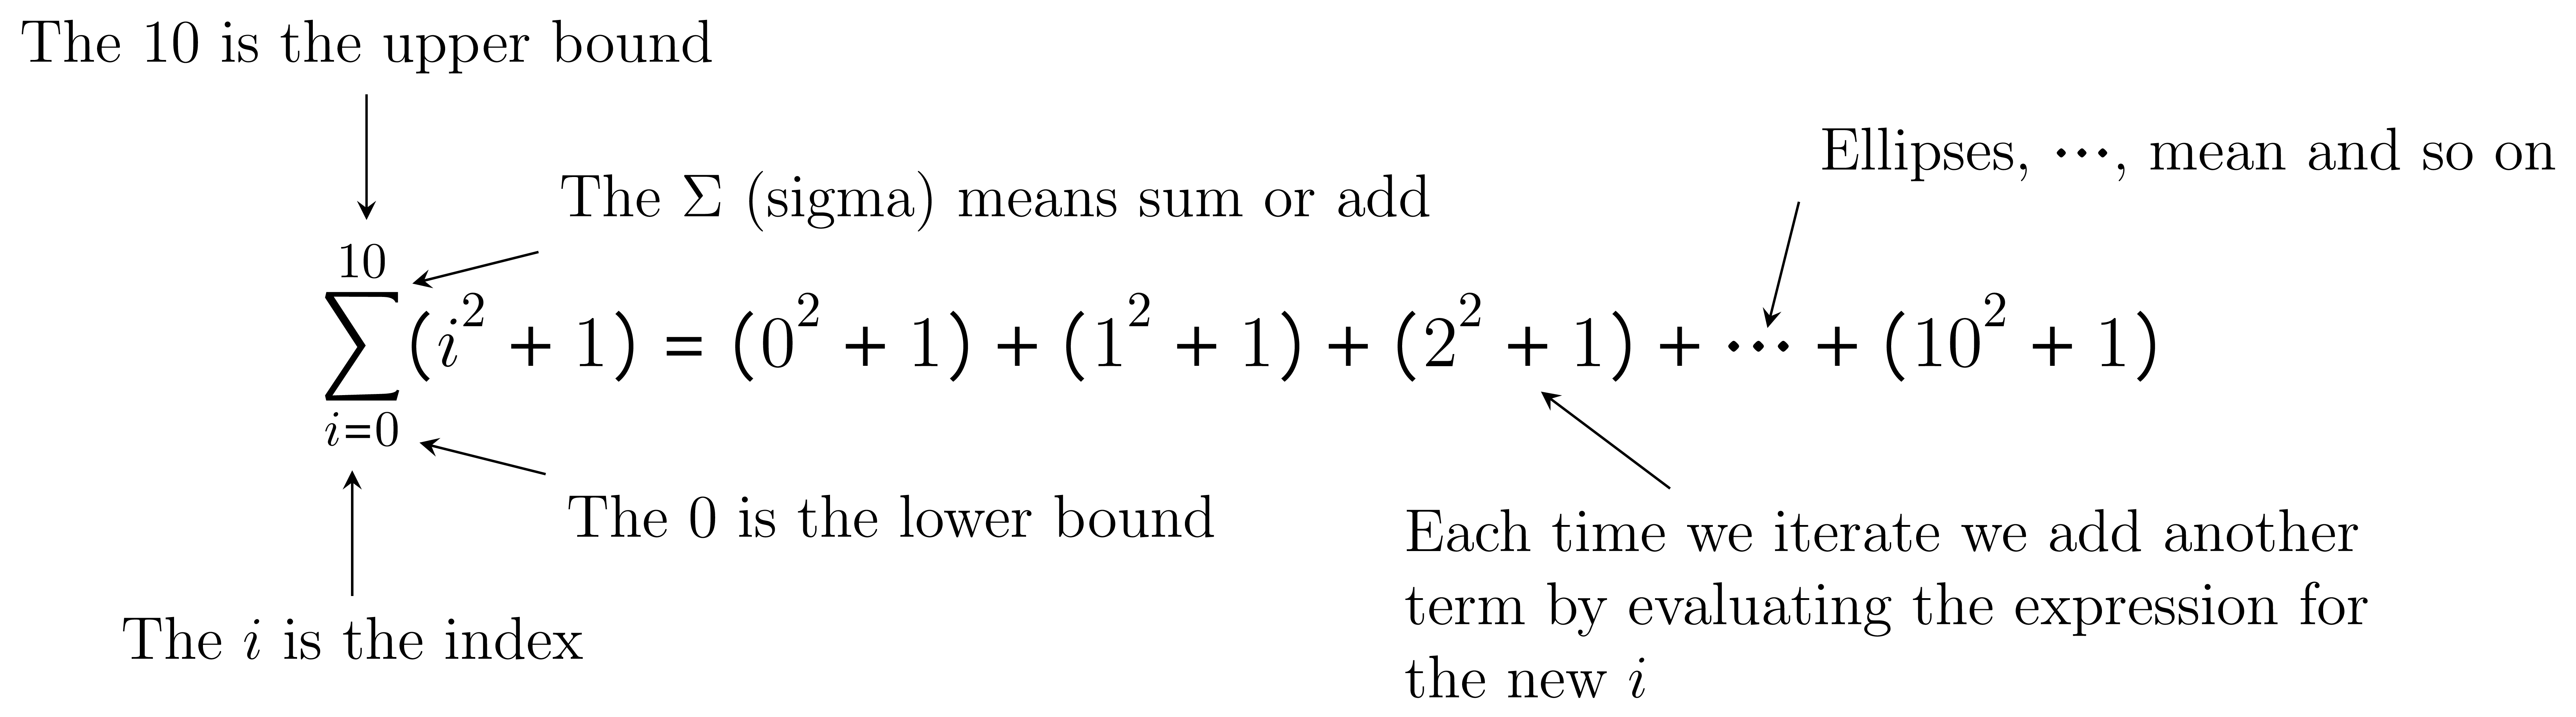
\includegraphics[scale=0.05,alt={Example of summation notation with lables for the various components of the notation}]{images/created/summation_notation.png}
    \caption{Summation Notation}
    \index{summation notation}
    \label{fig:sum_notation}
\end{figure}
\index{summation}
\end{defn}

\begin{defn}[Product]
A \emph{product} of terms in a sequence \(a_k\) can can be written 
    \[\prod_{i=0}^n a_i = a_0\times a_1\times a_2\times\cdots\times a_n\]
and is read ``the product from \(i\) equals zero to \(n\) of \(a_i\).''  For example in figure \ref{fig:prod_notation} we are multiplying terms in the sequence \(a_k=k^2+1\) and we would read it as ``the product from \(i\) equals zero to 10 of \(a_i=i^2+1\).''
\begin{figure}[H]
    \centering
    % \inputtikz{product_notation}
    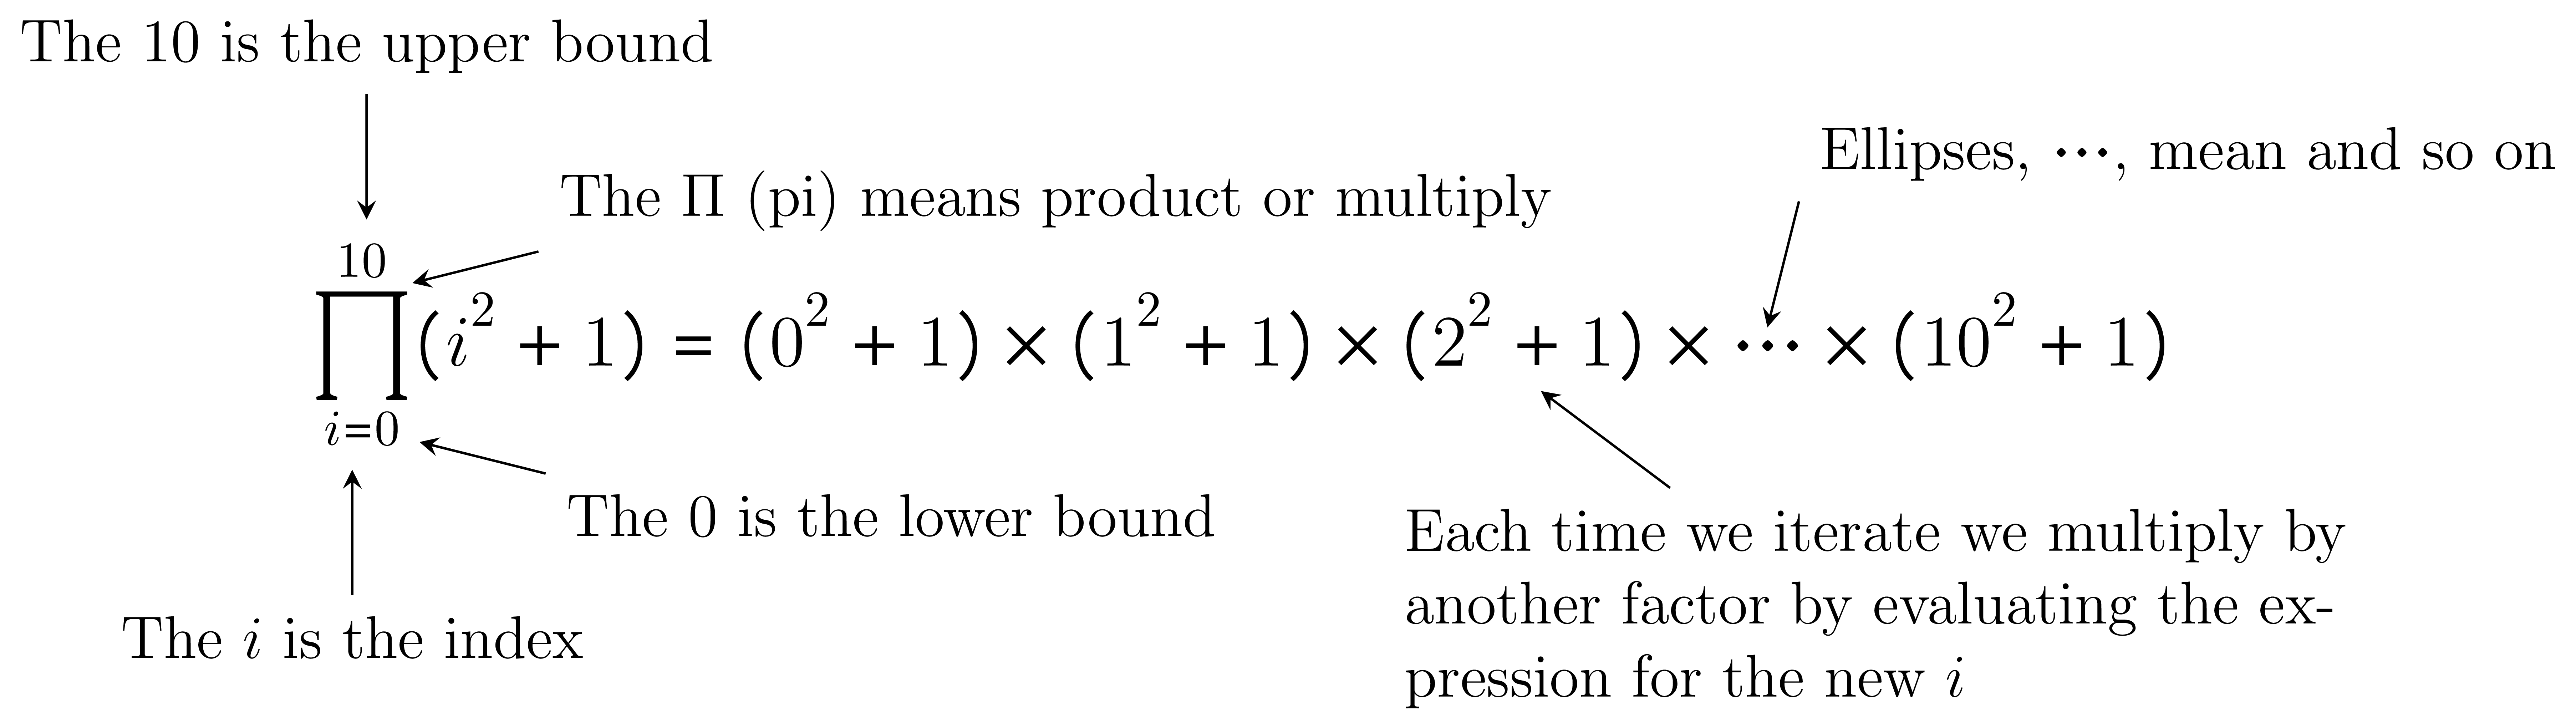
\includegraphics[width=0.85\linewidth,alt={Example of product notation with lables for the various components of the notation}]{images/created/product_notation.png}
    \caption{Product Notation}
    \index{product notation}
    \label{fig:prod_notation}
\end{figure}
\index{product}
\end{defn}
